\documentclass[twocolumn, a4paper, 12pt]{article}
\usepackage{graphicx} % Required for inserting images
\graphicspath{{./images/}}
\usepackage{float}  % For [H] option to control figure placement
\usepackage[
backend=biber,
style=numeric,
sorting=ynt
]{biblatex}
\addbibresource{references.bib}

\title{Evolutionary Optimization of Boid Flocking Behaviour using Genetic Algorithms}
\author{Ahmed Abdelhaleem \\ University of Sussex}
\date{March 2025}

\begin{document}

\maketitle


\begin{abstract}
  Boid simulations model the flocking behaviour of birds, fish, and other swarm organisms through 3 simple interaction rules: cohesion, separation, and alignment. In this project, Genetic Algorithms (GA) are used to evolve optimal boid behaviours by adjusting these rule parameters. A fitness function evaluates the flocking performance based on the weights of cohesion, separation, alignment, and energy efficiency. Through iterative selection, mutation, and crossover, the flocking characteristics are improved over many generations. The results demonstrate that evolved boids exhibit more stable, cohesive, and adaptive flocking patterns than manually selected tuned parameters. This approach can be used in swarm robotics, collective AI behaviour, and autonomous multi-agent systems.
\end{abstract}

\tableofcontents   % Table of Contents
\listoffigures     % Table of Figures


\section{Introduction}
Flocking behaviour emerges from simple rules followed by individual agents, which are called "boids". Craig Reynolds' Boid model (1986) defines three primary behaviours: cohesion (sticking together with the neighbouring boids), separation (avoiding collisions with neighbouring boids), and alignment (matching direction of neighbouring boids) \cite{reynolds1987flocks}. Although manually tuning the weights of these behaviours can lead to realistic flocking, evolutionary computation provides a much more data-driven approach to optimising them. In this project, Genetic Algorithms are used to evolve the boid behaviour for a better collective and natural looking flocking motion.

Boids is an artificial life computer programme that outputs very realistic simulations of how birds, sheep, or fish flock together. Each "boid", short for "bird-like object", follows just 3 simple rules, yet the result looks surprisingly lifelike.

The fitness function is evaluated on the basis of the weights of cohesion, separation, alignment, and energy efficiency. Real flocks try to conserve energy while flying, walking, or swimming together, by making smooth adjustments to their movement patterns. They don't make sudden jerky movements unless they have to, because that wastes energy. The fitness function rewards the flock for efficient and gradual changes in speed and direction, and conversely penalises the flock for sharp movements, which can be observed in if the acceleration was too high. In other words, it is like giving each boid a score based on how "gracefully" they fly.

The significance of this research lies in its potential applications in swarm robotics, crowd dynamics, and decentralized AI systems. By evolving boid behaviour instead of using hardcoded parameters, a more adaptable and efficient agent-based models that self-optimise over time can be developed.


\section{Methods}
1. Boid Simulation

A boid simulation was implemented, where agents move in a 3D space using the VPython library implemented in Python, following Reynolds' rules. The behaviour of each boid is governed by four main weighted parameters:

    1. Cohesion Weight: Attraction to neighbours.
    
    2. Separation Weight: Avoidance of nearby agents.
    
    3. Alignment Weight: Matching velocity with neighbours.
    
    4. Energy Efficiency Weight: This score measures how economically the boids move by penalizing excessive acceleration.


2. Genetic Algorithm Implementation

    • Initialisation: We generate a population of boid parameter sets (randomised).
    
    • Fitness Evaluation: The fitness function scores each set based on the weights of the following parameters:
    
        o Cohesion: Distance variance among boids
        
        o Separation: Avoidance of close collisions
        
        o Alignment: Average velocity alignment
        
        o Energy Efficiency: How efficiently the flock moves

    • Mutation: Small, random changes in parameters ensure diversity.

    • Crossover: Pairs of set of parent boid parameters are combined at random points to create offspring, blending traits of both parents to potentially improve flocking behaviour.
        
    • Selection \& Reproduction: The sets of highest-performing boids undergo crossover and mutation.

    The above evolution process is repeated for multiple generations, having the goal to optimise the parameters and trying to increase the fitness function. In the implemented code, the evolution process was repeated for 150 generations.

\subsection{Fitness Function and its Parameters}
The fitness function is calculated based on the score of the four main parameter weights.

1. Cohesion Score: Measures how well the flock stays together, by calculating the centre of mass of all boids. Higher score means that the boids are closer to the centre of mass of the flock.

2.Separation Score: Ensures boids maintain safe distances from each other. Uses a minimum safe distance of 0.5 units, and a penalty to the fitness function is applied if boids get too close to each other. Higher score for this weight means that boids maintain proper spacing between each other.

3. Alignment Score: Measures how well boids are moving in the same direction, by calculating the average velocity of the flock. Higher score means that the boids are flying in similar directions.

4. Energy Efficiency Score: Rewards boids for smooth, efficient movement. Less acceleration means higher score, which encourages natural, flowing movement.

It is worth mentioning that the Energy Efficiency Score is weighted at just 20\% of the total fitness, as compared to 100\% of any of the other three parameters (cohesion, alignment, and separation).

The energy weight of 20\% was chosen as a moderate value that is significant enough to influence behaviour without dominating it. In addition to keeping the energy efficiency as a secondary priority behind the three core flocking behaviours (separation, alignment, and cohesion), which allows for noticeable but not excessive smoothing of movement.

The final fitness score is calculated by combining all these components together. Then the weights for each component evolve over time through the genetic algorithm, helping find the optimal balance between these behaviours.

\subsection{Simulation Environment}
Boids are created inside a red cuboid of size 12*9*9 units. 60 boids are initialised inside the cuboid borders through assigning random positions and velocity for each individual boid. The boids can roam freely inside the borders of cuboid, but cannot fly out of the borders of the cuboid. In case a boid crosses one of the borders, close to one of the corners, it will re-spawn at another corner.


\section{Results and analyses}
\subsection{Experiment Parameters}
The simulation enforces strict velocity and force constraints on each boid. The maximum speed of 0.1 units per frame prevents unrealistically rapid movement while the minimum speed of 0.05 units ensures boids maintain continuous motion rather than appearing to hover.

A maximum steering force of 0.01 units limits how sharply boids can turn or accelerate, promoting smoother, more natural movement patterns.

A neighbourhood radius of 2.5 units was used in this simulation. It determines how far each boid can see and interact with other neighbouring boids. This value was chosen to create realistic flocking behaviour, as it creates a good balance between local and global awareness, similar to how real birds react to their immediate neighbours rather than the entire flock.

\subsection{Experiments and analyses}
The simulation runs at 60 frames per second. The evolution takes place every 60 frames, so the genetic algorithm evolves the four main parameters every second.

It is clear from the plot of the fitness score versus the number of generations (evolution steps), that the fitness score increases by increasing the number of generations. As can be seen in Figure \ref{fig:1}.

\begin{figure}[H]
    \centering
    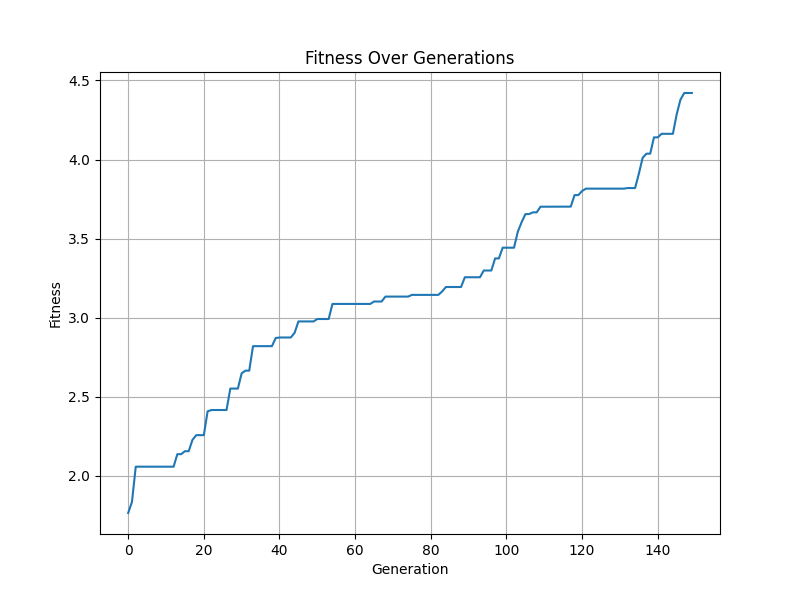
\includegraphics[width=0.9\linewidth]{fitness_vs_generations.png}
    \caption{Fitness Vs No. of Generations}
    \label{fig:1}
\end{figure}

The following plot shows the variation in the four main parameters, created by the mutation, crossover, and selection by the genetic algorithm. As can be seen in Figure \ref{fig:2}.

The best weights that were obtained are 1.972 for the separation weight for the alignment weight, 1.42 for the cohesion weight, and 0.902 for the energy weight.

\begin{figure}[H]
    \centering
    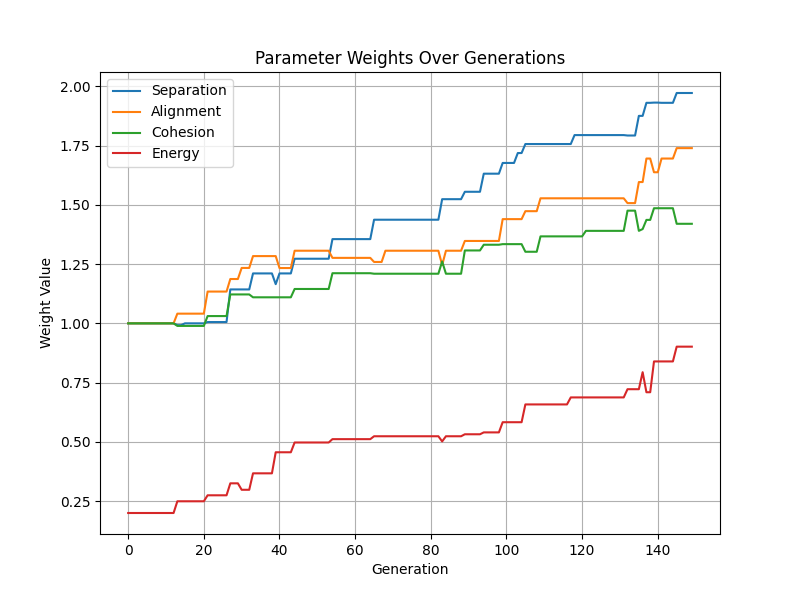
\includegraphics[width=0.9\linewidth]{images/parameter_weights.png}
    \caption{Parameter Weights Vs No. of Generations}
    \label{fig:2}
\end{figure}

It is clear from the simulation that the best fitness (peak value) is obtained at the end of the $150^{th}$ generation, having a value of 4.421. As can be seen in Figure \ref{fig:3}.

\begin{figure}[H]
    \centering
    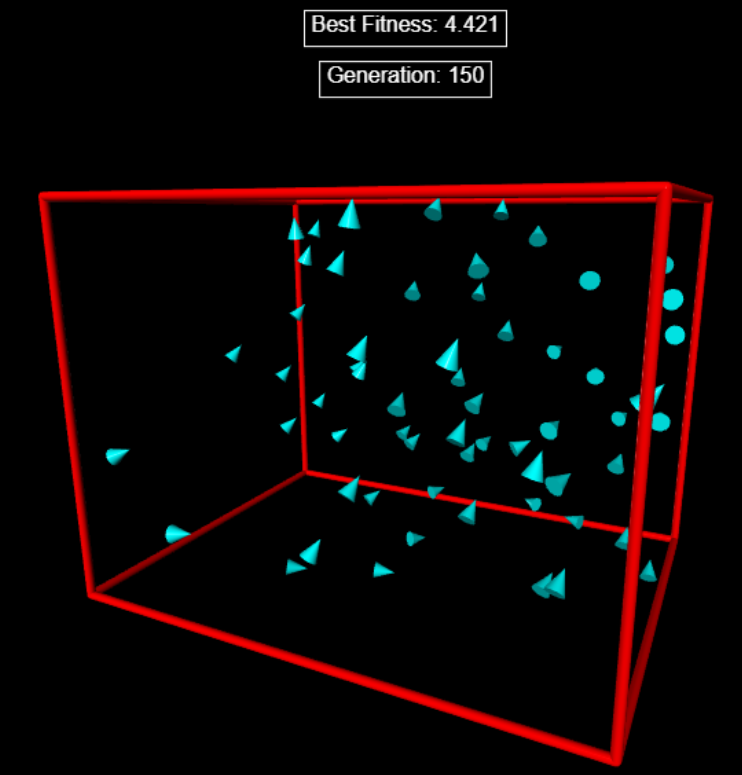
\includegraphics[width=0.8\linewidth]{simulation.png}
    \caption{3D Simulation}
    \label{fig:3}
\end{figure}

After running simulations for a selected number of 150 generations:

• Improvement in Flocking Behaviour: Initial random boids displayed chaotic motion, while evolved boids formed stable and structured flocks.

• Reduced Collision Frequency: The separation weight was self adjusted to avoid overcrowding.

• Better Alignment: Higher scoring generations showed improved velocity matching.

• Adaptive Flocking: The evolved boids dynamically responded to environmental changes.

One interesting observation: After running the genetic algorithm for 200 or more generations, the fitness score continued to increase as expected. However, the 3D visualisation revealed unnatural, extremely sharp, and jittery movements for the boids, that were visually off-putting. This shows how visualisation is important alongside the fitness function. In the example of boids, relying 100\% solely on optimizing the fitness function without considering the natural flow of the simulation can lead to unrealistic and undesirable behaviour.


\section{Discussion}
This research can be further expanded by a multitude of ways; one way would be to explore a broader range of weights beyond the weights that have been used in the fitness function of this study, which are how well the 3 main rules are being applied, which are separation, cohesion, alignment, in addition to the energy conversation based on the acceleration. Velocity Variation and Subgroup Formation are great examples when it comes to studying other interesting parameters to be used in a new fitness function.

Velocity Variation, is rewarding flocks that show some natural speed variations rather than the entire flock moving at max speed. Subgroup Formation, encourages the formation of smaller subgroups within the flock, for a more natural looking flocking behaviour.

By deeply tapping into these parameters, a better understanding of boids behaviour can be obtained, thus helping to further optimise adaptive flocking patterns in virtual simulations or real life applications, such as swarm robotics, collective AI behaviour, and autonomous systems consisting of multiple agents.

One study optimised the Boids swarm model using Particle Swarm Optimization (PSO) and Genetic Algorithm (GA). The results show that PSO outperforms GA in speed and efficiency, achieving natural movement faster. While GA finds global optima, its higher computational cost makes PSO better for real-time applications, highlighting its efficiency in dynamic swarm simulations. \cite{optimisation}

Building on PSO's efficiency, Cui and Shi's introduced Boid Particle Swarm Optimization (BPSO), which enhances the standard PSO algorithm by integrating alignment and cohesion rules from Reynolds' model, aiming to improve optimization performance. BPSO operates in two distinct phases: an initial divergent phase, where particles adjust their trajectories based on alignment and cohesion, and a subsequent convergent phase that employs standard PSO update equations. This structured approach seeks to balance exploration during optimisation. Benchmark tests indicate that BPSO outperforms traditional PSO in solving complex problems.\cite{extra_optimisation}

Conley’s study uses a Genetic Algorithm (GA) to optimise boid behaviour for geographic cluster detection. Boids search datasets for clusters, but tuning their parameters is complex. GA improves configurations over previous heuristics but doesn’t always converge to a single solution. While effective, GA is computationally expensive. Future work aims to derive dataset-based rules to reduce reliance on optimisation. \cite{Conley2005EvolvingBU}

Another research extended the Boids model for fish schools by adding behaviours like following food, avoiding obstacles, and evading predators. A Genetic Algorithm (GA) optimises behaviour coefficients, improving realism. Results show GA enhances movement, making it more natural, though tuning complexity increases with more rules. \cite{boids_ga}

Recent advancements in swarm optimisation uses Bayesian Optimisation methods, as seen in BOIDS, which integrates PSO-inspired incumbent-guided search with adaptive subspace embeddings. This improves efficiency in high-dimensional spaces, complementing previous work on both GA and PSO in optimising Boids behaviour. BOIDS’ structured approach enhances exploration-exploitation balance, which shows potential for hybrid models combining swarm intelligence with probabilistic optimization.\cite{future}

The results from this research demonstrate the effectiveness of Genetic Algorithms in optimising agent-based systems. By evolving rule parameters instead of manually setting them, we enable adaptive behaviour that outperforms traditional heuristic approaches. Future work could extend this method to environments with obstacles, or real-world robotic applications. Furthermore, reinforcement learning could also be used to optimise the behaviour of boids dynamically.

This research underscores the power of evolutionary computation in multi-agent
coordination and swarm intelligence, paving the way for autonomous and decentralised collective behaviour.


\section{Bibliography}
\printbibliography[heading=none]

\end{document}